\documentclass[../Report.tex]{subfiles}

\begin{document}


\chapter{Test}
\label{chap:test}

\section{---- firstName ----}
\label{sec:test_firstName}

\begin{figure}[H]
\centering
\tikzstyle{block_g} = [rectangle, draw, fill=green!20, 
    text width=6.5em, text centered, rounded corners, node distance=2cm, minimum height=4em]
\tikzstyle{block_b} = [rectangle, draw, fill=blue!20, 
    text width=6em, text centered, rounded corners, node distance=4.5cm, minimum height=4em]
\tikzstyle{block_r} = [rectangle, draw, fill=red!20, 
    text width=6em, text centered, rounded corners, node distance=4.5cm, minimum height=4em]
\tikzstyle{line} = [draw, -latex']
\begin{tikzpicture}[node distance = 5cm, auto]
    % Place nodes
    \node [block_g] (ideal) {$\Uout_{,\textrm{ideal}}$ festlegen};
    \node [block_g, below of=ideal] (H) {$\Hcompl$ bestimmen};
    \node [block_g, below of=H] (K) {$K_0$ bestimmen \newline Ref.: \newline ${V_{PP,?} = \SI{600}{\mV}}$};
    \node [block_b, right of=H] (Uquest) {$\Uquest_{,\textrm{ideal}}$ berechnen};
    \node [block_b, below of=Uquest] (Uin) {$\Uin$ berechnen};
    \node [block_r, right of=Uquest] (adjust) {$\Hcompl$ anpassen $H_i$ neu berechnen};
    \node [block_b, right of=Uin] (Uout) {$\Uout$ messen};
    
    % Draw edges
    \path [line, thick] (ideal) --  (H);
    \path [line, dashed] (H) -- node {$\Hcompl_0$} (Uquest);
    \path [line, thick] (H) -- (K);
    \path [line, thick] (K) -- node {$K$} (Uin);
    \path [line, thick] (Uin) -- (Uout);
	\path [line, thick] (Uout) -- node {$\Uout_{,\textrm{meas}}$}(adjust);
    \path [line, thick] (adjust) -- node {$H_i$}(Uquest);
    \path [line, thick] (Uquest) -- (Uin);
    \path [line, dashed] (Uquest) -- ++(0,15mm) -- node {$\Uquest_{,\textrm{ideal}}$} ++(45mm,0) -- (adjust);
\end{tikzpicture}
\caption{Algorithmus zur Optimierung von $\Hcompl$}
  	\label{fig:Algorithmus.H}
\end{figure}



Diese Zeile teste das paket $ nameref$ mit \nameref{chap:test} und hier mit einer PHANTOMSECTION via \nameref{pha:test.try}---

%\begin{figure}[htb]
%\begin{center}
%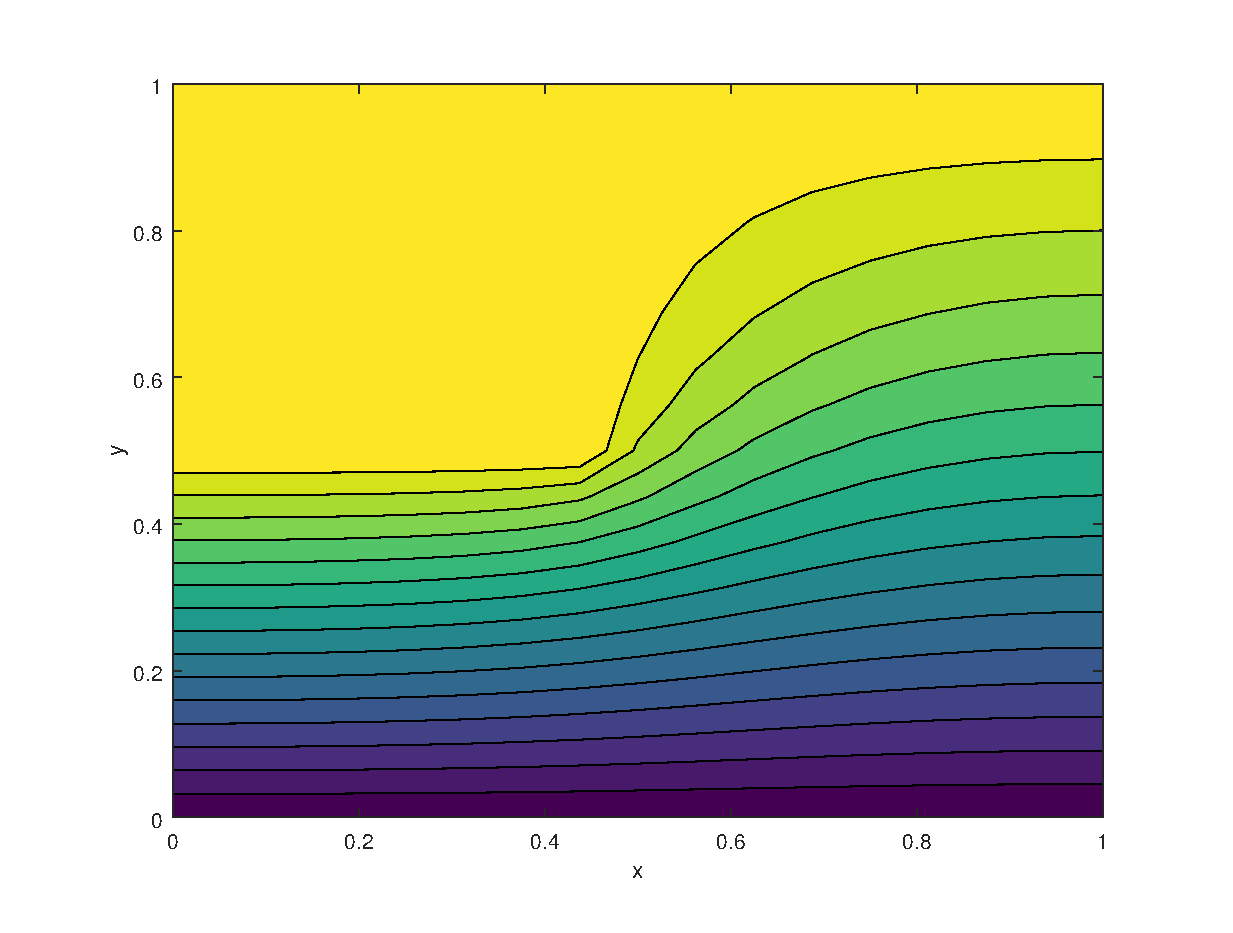
\includegraphics[scale=0.6]{eps/plotPot}
%\end{center}
%\caption[Potentialverlauf eines Kondensators mit Kante]{Potentialverlauf des Kondensators mit Kante.}
%\label{fig:V4.PA4.1}
%\end{figure}
%
%\begin{figure}
%	\centering
%	\begin{tikzpicture}[scale=1]
%		\begin{axis}[
%		xlabel={x},
%		ylabel={mode},
%		%grid=major,
%		cycle multi list={color list\nextlist [1 of]mark list},
%		legend entries={Grundmode},
%		legend style={at={(0.5,-0.2)},anchor=south},
%		]
%		\addplot table[x=x, y=mode1, col sep=comma] {../csv/modes.csv};
%		\addplot+
%%		\addplot+ [
%%mark=ball,
%%mark size=4pt,
%%scatter,% enable scatter
%%scatter src=rand,% the "color data"
%%% configure individual appearances:
%%scatter/use mapped color=
%%{ball color=mapped color}]
%coordinates
%{(-0.1,0) (-1,0.1) (0,0) (0.1,0.1) (0.2,0)};
%
%		
%		
%		\end{axis}
%	\end{tikzpicture}
%	\caption{asdf}
%\end{figure}
%
%
%
%\pgfplotstableread[col sep = comma, columns/3/.style={string type}, ignore chars= {(, ),j}] {transfer_fct.csv}\kennlinie %%%%% cannot deal with a 'j' in imaginary part! %%%
%%\pgfplotstabletypeset[columns={0,3}, columns/3/.style={string type}] \kennlinie
%% erzeugt eine banale Liste
%
%\begin{figure}[hb]
%\centering
%    \begin{tikzpicture}
%\begin{axis}[
%		legend entries = {Amplitude},
%		legend pos = outer north east,
%		extra y tick ={5}
%		extra y tick labels={hier ist $5$}
%		]
%\addplot[blue, thick] table [ x =0, y index=1] {\kennlinie};
%
%		\addplot [red, mark=o, mark size=5pt]coordinates {(10000000, 8)};
%		\addplot coordinates{(20000000, 5)}	;	
%		
%\end{axis}
%\end{tikzpicture}
%\caption{Einzelsinus}
%\end{figure}
%
%Dies ist ein Versuch, eine Transfer-Function zu plotten mittels tikz:

%\begin{figure}[h!]
%\centering
%    \begin{tikzpicture}
%    \datavisualization [scientific axes=clean, 
%    					visualize as line, 
%    					x axis = {attribute = frequency},
%    					y axis = {attribute = amplitude}]
%    	data [read from file = transfer_fct.csv,
%    			%headline = {frequency, amplitude, phaseshift, complex}
%    			];
%    
    
%\begin{axis}[grid=both, xlabel={$t/T_{\textrm{BB}}$},
%ylabel={$\Usin(t)$},                        ytick={-1,1},
%                        yticklabels={$-\widehat{U}$,$\widehat{U}$},
%                        xtick={-4,-2,0,2,4},
%                        xticklabels={-2,-1,0,1,2}]
%\addplot[blue, thick] table [ x expr={\thisrowno{0}}, y
%expr={\thisrowno{1}}, col sep=semicolon] {csv/transfer_fct.csv};
%\end{axis}
%	\end{tikzpicture}
%\caption{Bsp-Plot einer Transfer-Function H}
%  \label{fig:bsp_transfer}
%\end{figure}

%
%Dies ist ein Versuch, ein Frequenzspektrum zu plotten und Marker an relevanten Punkten zu setzen: Hiermit soll die Refernz in Sub-figures versucht werden:
%Dies hier soll zu \ref{fig:opt.spektrum_BB_signal} dem Hauptbild referenzieren.\\
%Dies hier soll zu \ref{fig:opt.abs_spektrum} dem Betragsspektrum referenzieren.\\
%Dies hier soll zu \ref{fig:opt.angle_spektrum} dem Phasen referenzieren.\\
%
%
%\pgfplotstableread[col sep = comma] {f_abs_orig.csv} \fabsOrig 
%\pgfplotstableread[col sep = comma] {f_abs_RMS_1.csv} \fabsRMSone 
%\pgfplotstableread[col sep = comma] {f_abs_RMS_2.csv} \fabsRMStwo
%\pgfplotstableread[col sep = comma] {f_abs_RMS_3.csv} \fabsRMSthree
%\pgfplotstableread[col sep = comma] {H_RMS_orig.csv} \Horig
%\pgfplotstableread[col sep = comma] {H_RMS_1.csv} \HrmsOne
%\pgfplotstableread[col sep = comma] {H_RMS_2.csv} \HrmsTwo
%\pgfplotstableread[col sep = comma] {H_RMS_3.csv} \HrmsThree
% 
%
%\begin{figure}[htb]
%\caption[Ignorieren großer Korrektur-Terme]{Entwicklung von Übertragungsfunktion und Korrekturterm bei Beschränkung von $\fabs$}
%\label{fig:opt.spektrum_BB_signal}
%\begin{subfigure}{0.5 \textwidth}
%    \begin{tikzpicture}
%\begin{axis}[
%		legend entries = {original, Step 1, Step 2, Step 3},
%		legend pos = north east,
%		xlabel={Frequenz},
%		ylabel={Betrag Übertragung $\Hcompl$},
%		%xtick distance = 10000000,
%%		xminorgrids,
%%		xmajorgrids,
%%		minor x tick num =3,
%		xtick pos = lower,
%		ytick pos = left,
%		xtick align = outside,
%		ytick align = outside,
%		scaled x ticks = base 10:-6,
%		xtick scale label code/.code={[MHz]},
%		xmin = -5000000,
%		xmax = 85000000,
%%		ymin = 0,
%		%ymax = 0.03,
%		]
%		\addplot table [x index = 0, y index = 1] {\Horig};
%		\addplot table [x index = 0, y index = 1] {\HrmsOne};
%		\addplot table [x index = 0, y index = 1] {\HrmsTwo};
%		\addplot table [x index = 0, y index = 1] {\HrmsThree};
%\end{axis}
%\end{tikzpicture}
%\subcaption{ -- name ---}
%	\label{fig:opt.abs_spektrum}
%\end{subfigure}
%\begin{subfigure}{0.5 \textwidth}
%    \begin{tikzpicture}
%\begin{axis}[
%		legend entries = {original, Step 1, Step 2, Step 3},
%		legend pos = north east,
%		xlabel={Frequenz},
%		ylabel={Korrekturterm $\fabs$},
%		%xtick distance = 10000000,
%%		xminorgrids,
%%%		xmajorgrids,
%%		minor x tick num =3,
%		xtick pos = lower,
%		ytick pos = left,
%		xtick align = outside,
%		ytick align = outside,
%		scaled x ticks = base 10:-6,
%		xtick scale label code/.code={[MHz]},
%		xmin = -5000000,
%		xmax = 85000000,
%%		ymin = 0,
%%		ymax = 0.03,
%		]
%		
%		\addplot table [x index = 0, y index = 1] {\fabsOrig};
%		\addplot table [x index = 0, y index = 1] {\fabsRMSone};
%		\addplot table [x index = 0, y index = 1] {\fabsRMStwo};
%		\addplot table [x index = 0, y index = 1] {\fabsRMSthree};
%\end{axis}
%\end{tikzpicture}
%\subcaption{--- name --}
%\end{subfigure}
%\end{figure}


\end{document}